\chapter{Continuous measurements of \Ttwo and \SOtwo}
\label{ch:cont}
The continuous flow loop experiments were designed to address some of the shortcomings of the stopped flow experiments, including the difficulties associated with measuring intermediate levels of oxygenation, and the effects of red blood cells settling when stationary.
As mentioned in the introduction, measurements with continuously flowing blood have been demonstrated by Meyer\cite{MeyerNMRrelaxationrates1995} and the group of Peter van Zijl\cite{ZhaoOxygenationhematocritdependence2007,QinDeterminationwholebrainoxygen2011,GrgacTransversewaterrelaxation2017}.

The first step in this experiment was to confirm that \Ttwo can still be measured in a flowing sample, and to measure the effect of flow on the observed \Ttwo.
This was completed using a sample of water doped with CuSO\textsubscript{4} to give a \Ttwo similar to blood.
The stability of the flow rate in the circuit was also tested.

Following this, experiments with samples of blood were completed to measure \Ttwo at a range of echo times, while \SOtwo was slowly ramped between oxygenated and deoxygenated.
These experiments were completed at fields of \SIlist{0.1;0.2;0.3;0.5;1.0}{T} (corresponding to \SIlist{5;10;14;20;40}{MHz}) to investigate the field dependence of the \Ttwo shortening effect.

\section{Experimental Protocol}

In these continuous flow experiments, the samples of blood used were `fresher' than in the stopped flow experiments, to try and decrease any effects from haemolysis.
The samples were typically used less than 3 days after collection.
To prepare for the experiments, the blood was removed from the fridge and allowed to warm to room temperature while the flow circuit was assembled, and put into the magnet.
In most cases, the magnet was set to the correct magnetic field at least a day before (except for the 20 MHz experiment, which was run immediately after the 40 MHz experiment.)
The water bath controlling the gradient bore temperature was also turned on, this required approximately 40 minutes to warm up and stabilise.
As in the stopped flow experiments, the blood was loaded into the flow circuit, and warmed to the experiment temperature and oxygenated by flowing it through the oxygenator.
During this time, the probe was tuned and matched, and NMR parameters such as pulse power and phase were calibrated.
An initial sample with the iStat was measured, and a \SI{3}{ml} samples was taken for plasma separation in the centrifuge.
Plasma was separated by running the centrifuge at setting `5' for 15 minutes, then removing the plasma layer by pasteur pipette.

The flow rate was set by clamping the tube between the magnet and the lower blood bag.
Initially, the screw clamp was closed and the pgse-profile experiment was started.
The clamp was then loosened until a flow rate around \SI{1}{cm/s} was reached, measured using the phase shift from the NMR experiment.
After this was found, the screw clamp was not adjusted for the rest of the experiment, and the pump rate was set to compensate for the flow and keep a constant volume in both bags.

In these experiments the oxygenation level was slowly ramped down by flowing gas with 0\% \Otwo through the oxygenator while the circuit was flowing.
This flowed into the upper blood bag, where mixing with the oxygenated blood helped to smooth the change in \SOtwo and slow down the process, so that more data points could be collected as the oxygenation decreased.
In the first deoxygenation ramp at each field, samples of blood were taken for blood gas analysis on the iStat to calibrate the optical sensor, as discussed in \autoref{sec:exptsetup-pulseoximeter}.
This was done during deoxygenation, as we found that this had a slower rate than the oxygenation.

To oxygenate the blood, the gas mix through the oxygenator was changed to have 21\% \Otwo.
In later experiments, this was altered slightly to have a stage with 5\% \Otwo, followed by a stage at 21\% \Otwo.
This helped to slow down the oxygenation, and allow more data points to be collected.
Deoxygenation and oxygenation ramps were repeated at least twice for each field/sample.

\subsection{NMR Experiments}
To collect the CPMG and PGSE data, a looping batch script was set up in Prospa to automatically run the experiments.

Multiple versions of the standard CPMG experiment included in Prospa were added with echo times equal to \SIlist{1;5;8;10;20}{ms}, and the number of echoes varied to give a total echo train length of \SI{600}{ms}.
4 scans of each CPMG experiment were used with the standard phase cycling and a \SI{1.2}{s} inter-experiment delay (the sample was flowing through the coil, bringing in `fresh' spins, so the repetition time could be less than $5 \times \mathit{T_1}$.)
Additionally, a PGSE experiment was added to monitor the flow rate, with $\Delta = \SI{16}{ms}$, $\delta = \SI{2}{ms}$, $\mathit{g} = \SIrange{0}{0.015}{T/m}$ over 4 steps, and a \SI{15.5}{ms} echo time.
The x gradients were used as the PGSE gradient, as this corresponds to the direction of flow through the coil.

\begin{displaymath}
v = \frac{\phi}{\gamma \Delta \delta g}
\end{displaymath}
Using TODO background PGSEphase shift eq, these parameters allow for measurement of velocities \SI{< 5}{cm/s} without phase wrapping.
A standard 1pulse FID experiment is also run, to test for any shifts in the magnetic field.

The batch script in Prospa runs each experiment, then moves to a new directory and repeats.
Each cycle of 7 experiments takes approximately 45 seconds, to complete.
Data is also continuously collected from the optical \SOtwo sensor, and the Picolog temperature logger.

The data is processed using Python in JuPyter notebooks.
Each echo train is phased, and each echo is summed to give a single value for the signal at each echo time.
Similarly to the stopped flow experiments, signal before \SI{15}{ms} was trimmed before using non-linear fitting to get a \Ttwo value for each CPMG decay.
Additionally, the time of each CPMG experiment was extracted from the file system, so that it could be compared with the \SOtwo measurements.


\section{Results}
\subsection{\Ttwo and flow}
\label{sec:contflow-Ttwoflow}
Having the sample flow through the coil causes a decrease in the measured \Ttwo, due to the effect of added dispersion, and the outflow of excited spins from the coil.
In particular, the outflow effect becomes signifcant as the time in the coil (\SI{2}{cm} long) becomes shorter than the experiment time, as the decrease in spins from the coil adds to the true \Ttwo decay and causes the \Ttwo to appear shorter.
To test the impact of flow on the \Ttwo measurements in this experiment, a 1\% NaCl solution doped with \SI{5}{mmolL^{-1}} CuSO\textsubscript{4}, was prepared to test with.
This was loaded into a circuit without the oxygenator and CPMG and PGSE experiments were measured at a range of flow rates.

\begin{figure}[ht]
%Graph from processBloodOxygenation2/171116 Doped water twobag s1.ipynb
\centering
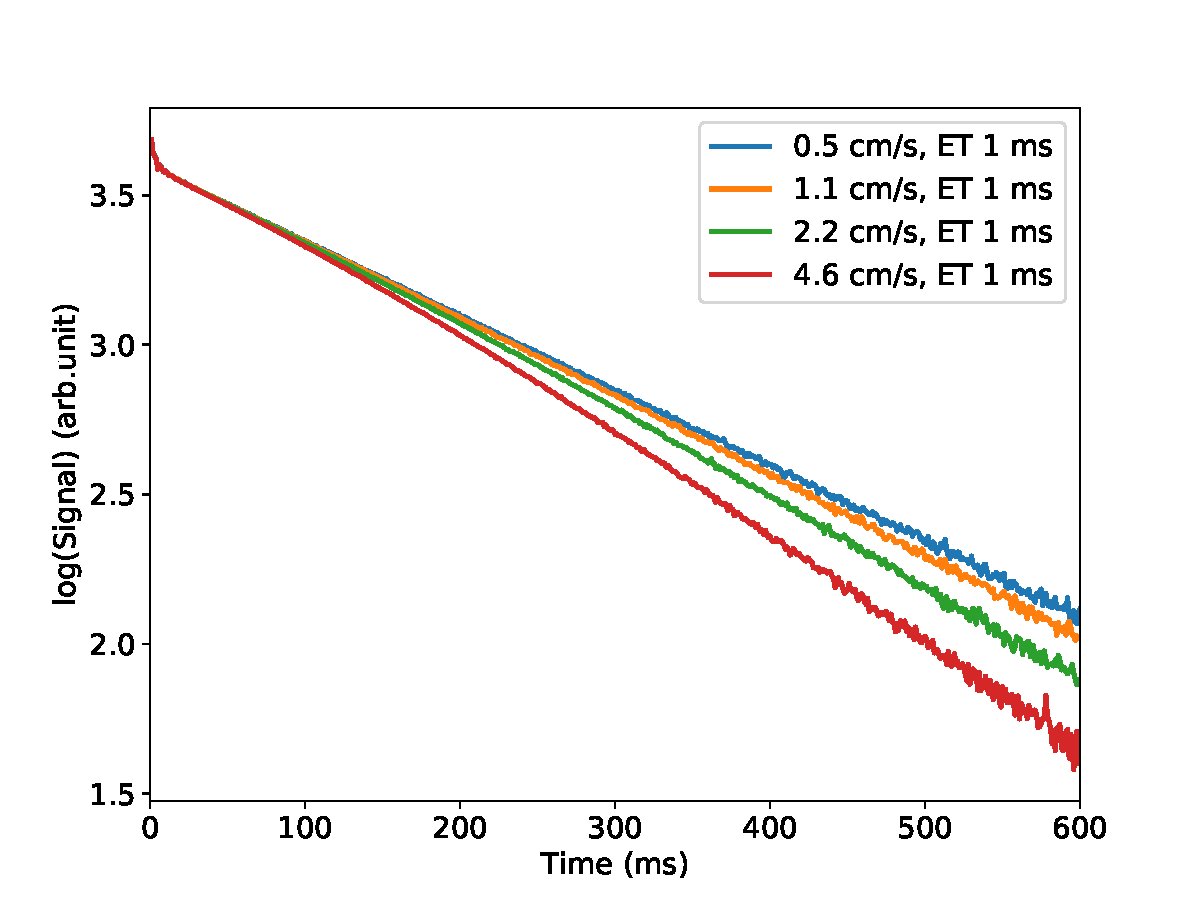
\includegraphics[width=0.8\textwidth]{figures/contflow/dopedwatercpmgdecay.pdf}
\caption{Examples of CPMG echo trains for doped water samples at different flow rates}
\label{fig:contflow-watercpmgdecay}
\end{figure}

\autoref{fig:contflow-watercpmgdecay} shows CPMG echo trains measured for the doped water measured at 4 flow rates, shown on a log scale.
In the first \SI{100}{ms}, all four decays appear the same, but as the flow rate increases, the lines become curved as the signal stops being monoexponential.
As expected, this effect is much larger at the highest flow rate (\SI{4.6}{cm/s}.)
Interestingly, this speed corresponds with a time in the coil of only \SI{430}{ms}, but signal is still being detected after this, suggesting that there is a distribution of speeds in the sample. TODO is this that propagator thing??
There appears to be little effect at the two lower flow rates, and at \SI{2.2}{cm/s}, the effect is not significant until approximately \SI{300}{ms} into the decay.
These decays were fitted with non-linear fitting to obtain \Ttwo values at different flow rates, shown in \autoref{fig:contflow-Ttwovelocity}.

\begin{figure}[t]
%Graph from processBloodOxygenation2/171116 Doped water twobag s1.ipynb
\centering
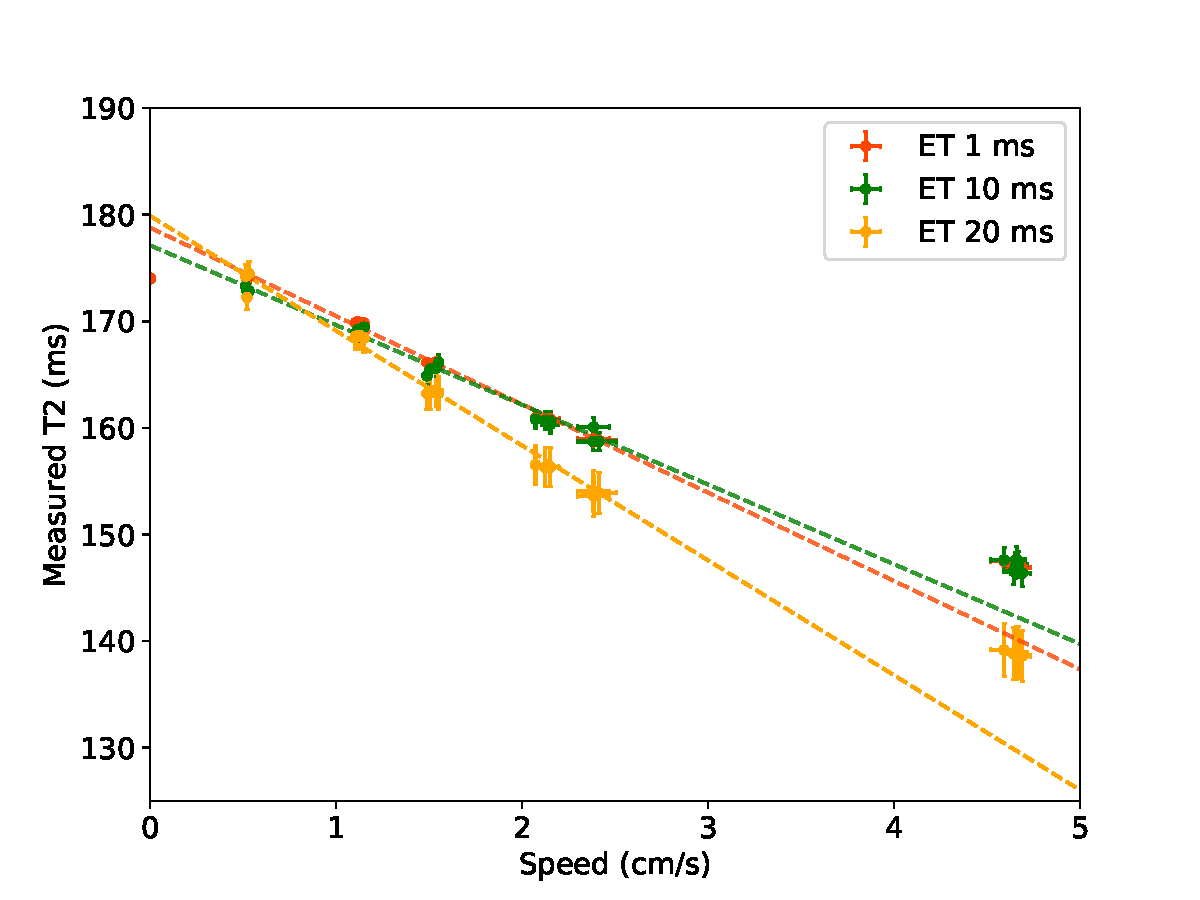
\includegraphics[width=0.8\textwidth]{figures/contflow/T2velocity.pdf}
\caption[Measured \Ttwo values at different flow rates]{Measured \Ttwo values at different flow rates. v=0 point measured in separate experiment. Lines fitted to points where v\SI{<3}{cm/s}.}
\label{fig:contflow-Ttwovelocity}
\end{figure}

As expected, the \Ttwo values measured at higher flow rates decrease from \SI{174}{ms} to around \SI{150}{ms}, with a stronger effect measured at the \SI{20}{ms} echo time.
The decrease appears roughly linear for all but the fastest speed, and these data points were fitted to determine the trend, and the intercept where v=0.
These fit parameters are included in \autoref{tab:contflow-Ttwovelocitylinfit}.

Because the \Ttwo decrease due to flow becomes negligible at low speeds (as the time in coil increases proportional to $\frac{1}{\mathit{v}}$), the intercepts of the lines of best fit overestimate the true \Ttwo (\SI{174}{ms}, measured in a separate experiment) by \SI{4}{ms}.
Additionally, the slopes would be dependent on the true \Ttwo of the sample, as a sample with a short \Ttwo would be less affected by the effect of flow, and vice versa.
As the \Ttwo of the blood will be changing during the experiment, applying the linear correction shown here would not necessarily work.

However, from these experiments, the change in \Ttwo due to flow should be less than \SI{10}{ms}, for flow rates less than \SI{1.5}{cm/s}.
To try and minimise the effect of flow, the section of the decay used to find \Ttwo was limited to the first \SI{360}{ms} of the echo train.
In blood \Ttwo changes due to blood oxygenation are larger than this effect -- on the order of \SI{50}{ms} at 10 MHz -- and the flow rate should stay relatively constant over the course of the experiment, so effects from flow should be relatively small.

\begin{table}[h]
\centering
\caption{Measured \Ttwo dependence on speed}
\label{tab:contflow-Ttwovelocitylinfit}
\begin{tabular}{|c|cc|}
\hline
Echotime (\si{ms}) & Intercept (\si{ms}) & Slope (\si{ms/cm/s}) \\
\hline
1        & 178 \pm 1    & -8.2 \pm 0.2    \\
10       & 177 \pm 1    & -7.4 \pm 0.3    \\
20       & 179 \pm 1    & -10.7 \pm 0.3  \\
\hline
\end{tabular}
\end{table}

\subsection{Flow stability}
\label{sec:contflow-flowstability}
The stability of the flow produced in the circuit was also tested, after early experiments showed a series of spikes in the \Ttwo data.

An example is shown in \autoref{fig:contflow-spikeyTtwo}, from an experiment with blood at 14 MHz.
There are large spikes of up to \SI{40}{ms} in the measured \Ttwo{}s, which makes it difficult to see trends due to changing \SOtwo.
Interestingly, there is a period of `calm' between 355 and 380 minutes, before it goes back to the random spike pattern.

\begin{figure}[ht]
%Graph generated in processBloodoxygenation2/171110 14mhz
\centering
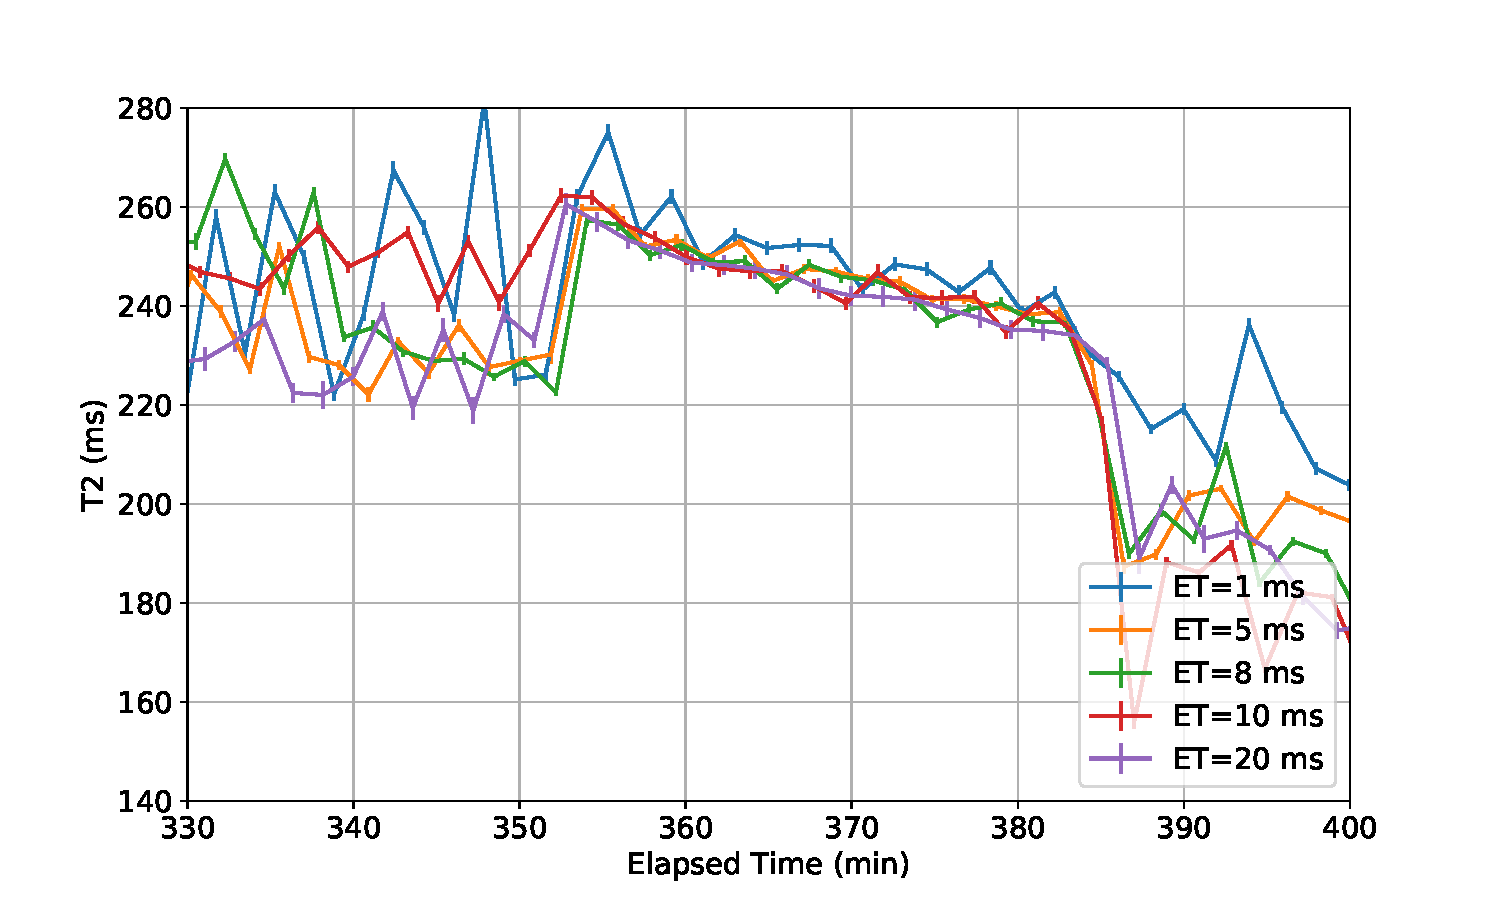
\includegraphics[width=\textwidth]{figures/contflow/spikeyTtwo.pdf}
\caption[Spikes in continuous \Ttwo measurements]{Spikes in continuous \Ttwo measurements from unstable flow}
\label{fig:contflow-spikeyTtwo}
\end{figure}

There were a number of possible causes for this effect, including absolute phase effects from the timing in the Kea spectrometer, and changing sauces of RF  noise.
This was eventually tracked down to an issue with the stability of the flow in the circuit.
In these experiments, the lower bag was not included in the circuit, so that the magnet output was connected directly to the peristaltic pump.
To see how this affected the flow circuit, PGSE experiments were used to measure the velocity of doped water sample flowing in the circuit.

\begin{figure}[ht]
%plots made in flowtesting round 2/fast pgseprofile pump
\centering
\begin{subfigure}[t]{0.32\textwidth}
\caption{No flow}
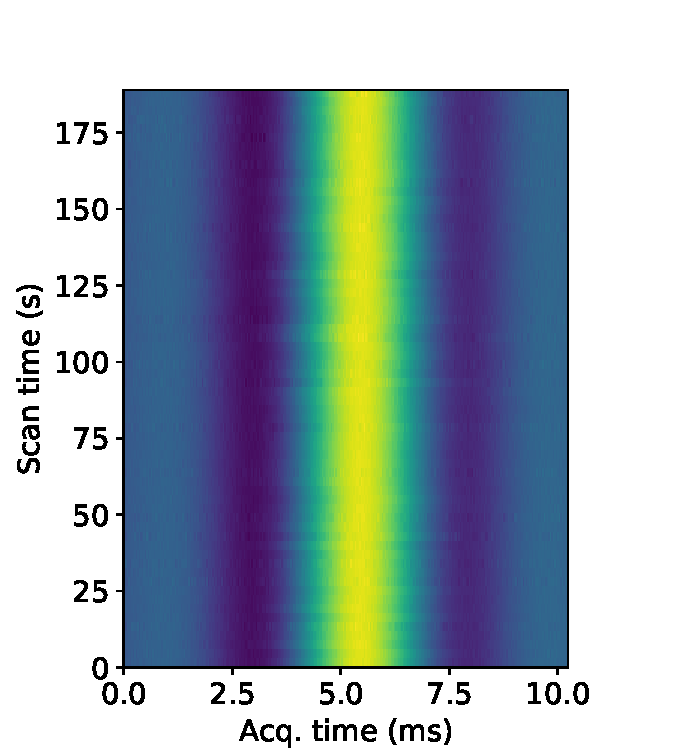
\includegraphics[width=\textwidth]{figures/contflow/flowstabilitynoflow.pdf}
\end{subfigure}
\begin{subfigure}[t]{0.32\textwidth}
\caption{Pump flow}
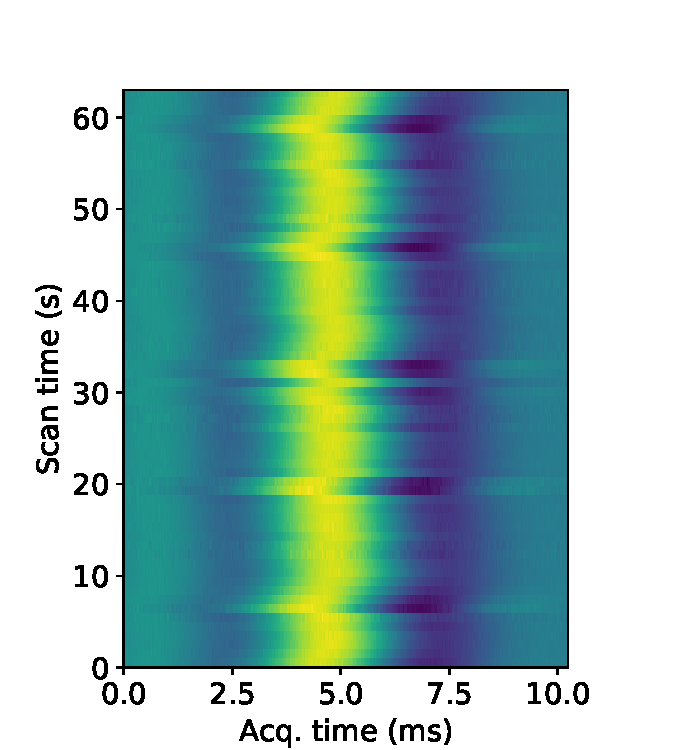
\includegraphics[width=\textwidth]{figures/contflow/flowstabilitybadpump.pdf}
\end{subfigure}
\begin{subfigure}[t]{0.32\textwidth}
\caption{Gravity flow}
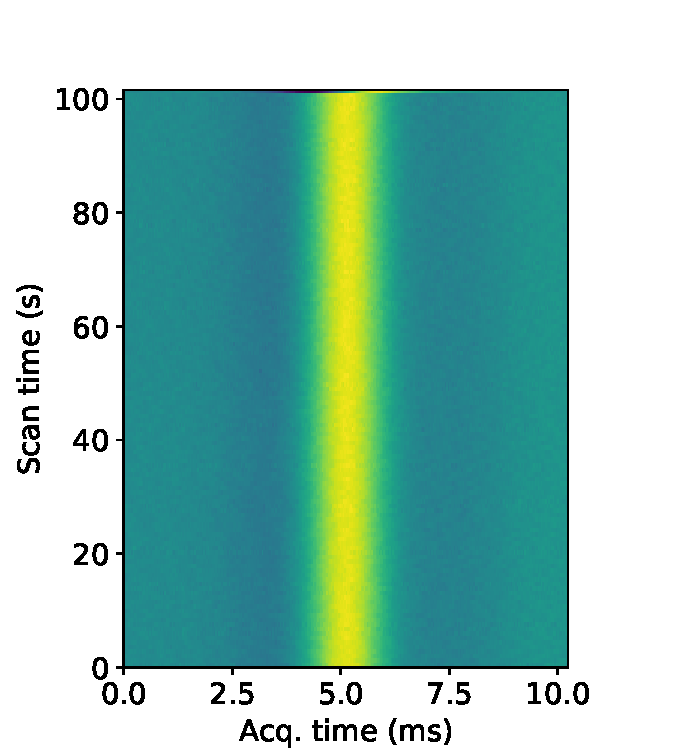
\includegraphics[width=\textwidth]{figures/contflow/flowstabilitynewsetup.pdf}
\end{subfigure}

\caption[PGSE data showing flow stability]{PGSE data showing stability for different flow setups. Collected with PGSE experiments using a repeated \textit{g/q} step so phase changes show velocity. The x-axis shows the acquisition time, while the experiment time is on y. Colour shows the intensity of the real part of the signal.}
\label{fig:contflow-flowstabilityrawpgse}
\end{figure}

\autoref{fig:contflow-flowstabilityrawpgse} shows the raw spin echoes collected in these experiments.
In this experiment, a constant value of \textit{g}=\SI{0.01}{T/m} was used so that changes in phase reflect changes in the velocity.
The experiment with no flow shows no changes in phase, as expected.
However, when the pump is turned on, there are clearly disturbances, which occur with a period of 13 seconds.
Processing this to find the velocities gives \autoref{fig:contflow-flowstabilityspeed}, which shows that the flow rate from the pump drops by over 50\% every 13 seconds.
This is half of the rotational period of the pump head (approximately 26 seconds when set to 2.3 rpm), which is expected as it has two rollers.
There is actually a short period of time where both rollers stop squeezing the tube, which could cause this instability.
When this is combined with the effect of phase cycling, this could cause the spikes in the measured \Ttwo.

The flow circuit was modified to include another blood bag between the magnet and the pump, and the have the blood flow under gravity.
This give a much more stable flow, as can be seen in \autoref{fig:contflow-flowstabilityrawpgse}(c), and the green curve in \autoref{fig:contflow-flowstabilityspeed}, which has a speed of \textit{v} = \SI{1.04\pm0.02}{cm/s} over the 100 seconds it was measured for.

\begin{figure}[ht]
%plots made in flowtesting round 2/fast pgseprofile pump
\centering
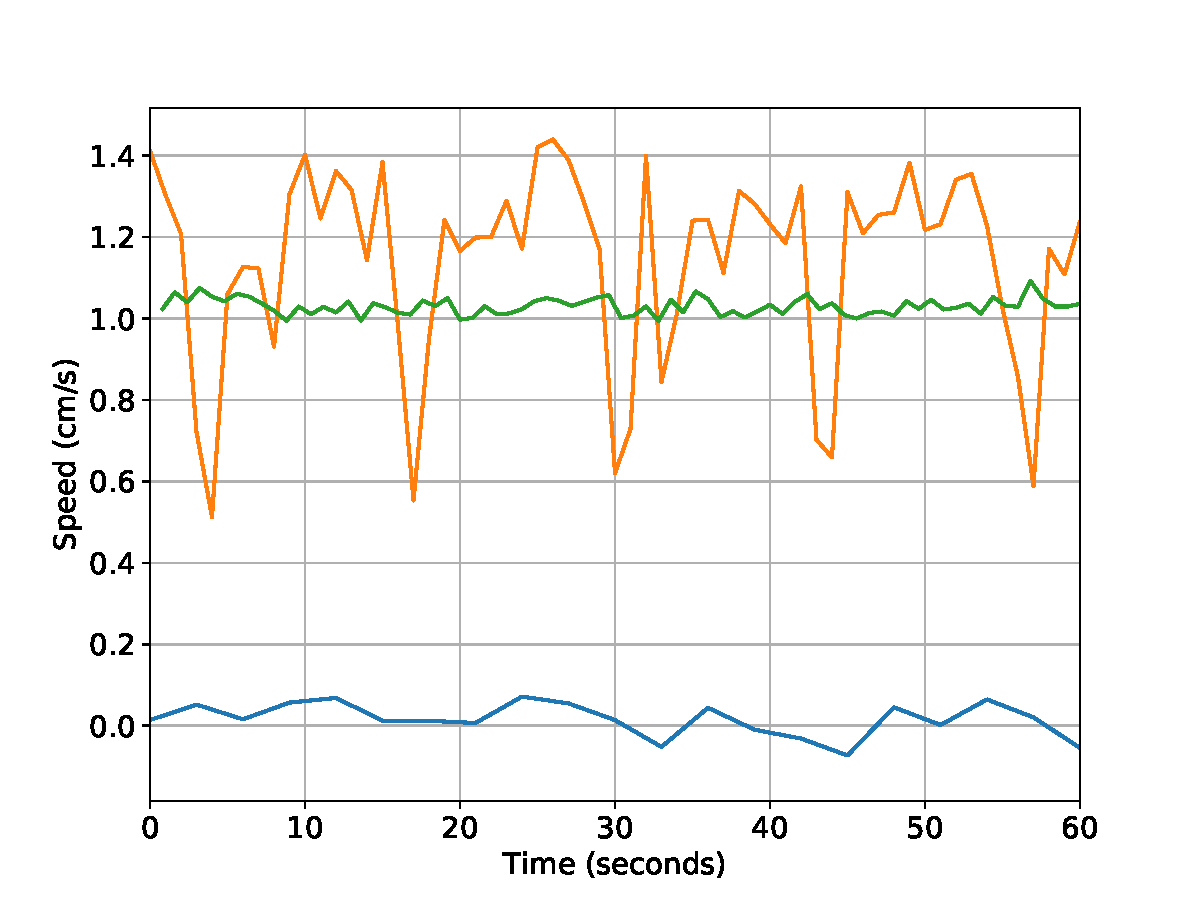
\includegraphics[width=\textwidth]{figures/contflow/flowstabilityspeed.pdf}
\caption[Flow rate stability for different continuous flow setups]{Flow rates measured by PGSE for: No flow (blue), Pump flow (yellow), Gravity flow (green)}
\label{fig:contflow-flowstabilityspeed}
\end{figure}

\begin{itemize}
\item Testing of \Ttwo change with flow
\item Flow stability, and pump pulsations - different
\item Experimental data - \Ttwo over time at diff fields
\item Graphs of \Ttwo vs \SOtwo change at 5 MHz, 10MHz, 14MHz, 20MHz, 40MHz
\item \Kzero to \SOtwo at diff fields
\end{itemize}

\section{Discussion}
\begin{itemize}
\item comparisons between different field strengths - agreement with literature
\item calibration of \Kzero to \SOtwo
\item mitigation of haemolysis
\item effect of blood velocity on \Ttwo

\end{itemize}
